\bghdr{images/fond-mac}

%\begin{center}
%
\includegraphics{images/logo_Mac}
%\end{center}



\subsection{Configuration sous Mac OS X}

La configuration est d\'etaill\'ee pour Mac OS 10.5 (\app{Leopard}). %et encore un peu pour Mac OS 10.4 (Tiger).
Afin de conna\^itre la version que tu utilises, va dans le \menu{menu Pomme} puis s\'electionne \menu{\`A propos de ce Mac}.

\subsubsection{Configuration IP}

\flimage{images/mac_prefs_icone}{0.07}{l}
 \app{Pr\'ef\'erences R\'eseau}, accessible depuis l'article de menu \menu{Pr\'ef\'erences syst\`eme} du menu \menu{Pomme}, permet de configurer la connexion au r\'eseau. Par ailleurs, si au d\'emarrage un assistant te propose de configurer ton r\'eseau, refuse et utilise la proc\'edure du BR. En effet, le r\'eseau n\'ecessite une configuration particuli\`ere  \`a l'X, plus complexe que celle effectu\'ee par cet assistant.


\noindent
  \begin{figure*}[h]
    \begin{center}  
     % \subfloat[Tiger]{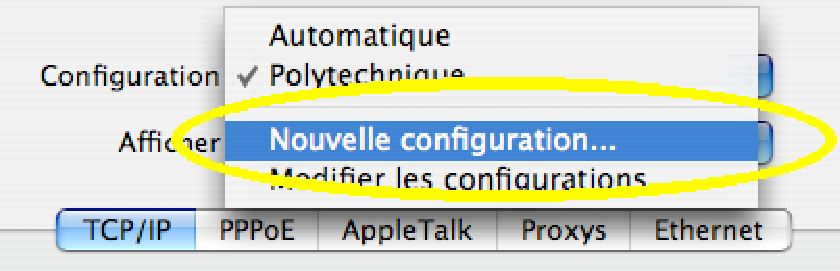
\includegraphics[width=0.47\textwidth]{images/mac_nouvelle_config} } 
     % \hfill
      \subfloat[Cr\'eer une nouvelle configuration r\'eseau]{ 
      \begin{minipage}{0.43 \textwidth}\begin{flushleft}
      {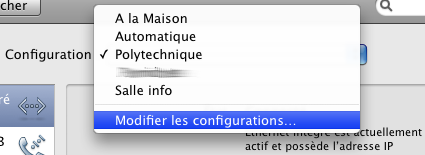
\includegraphics[width=0.96\textwidth]{images/mac_nouvelle_config_leopard_1}}\\ \vspace*{2cm}
      {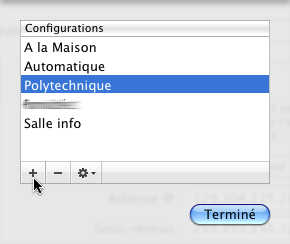
\includegraphics[width=0.96\textwidth]{images/mac_nouvelle_config_leopard_2}} 
 		\end{flushleft}  \end{minipage}
 		 } 		
 		\subfloat[Configuration de l'interface r\'eseau \emph{Ethernet}, de l'adresse IP et du \emph{proxy}]{ 
 		 \begin{minipage}{0.43 \textwidth}\begin{flushright}
 		{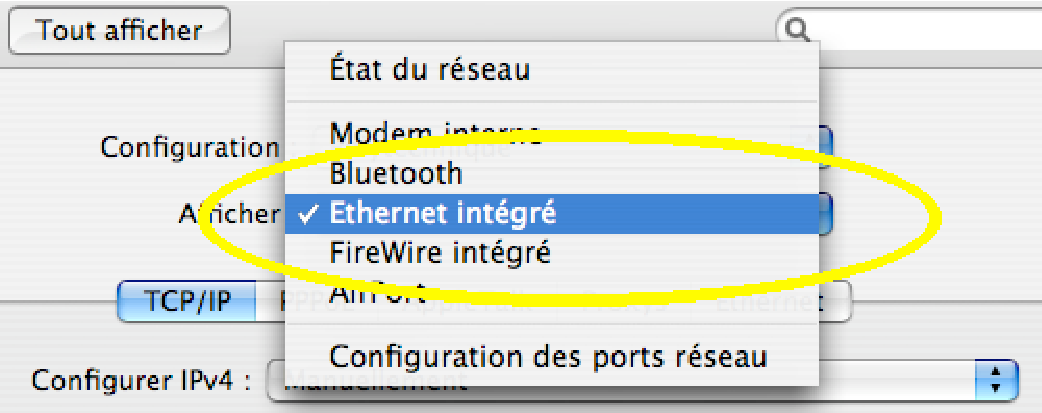
\includegraphics[width=0.96 \textwidth]{images/mac_config_ethernet}} \\ 
 		{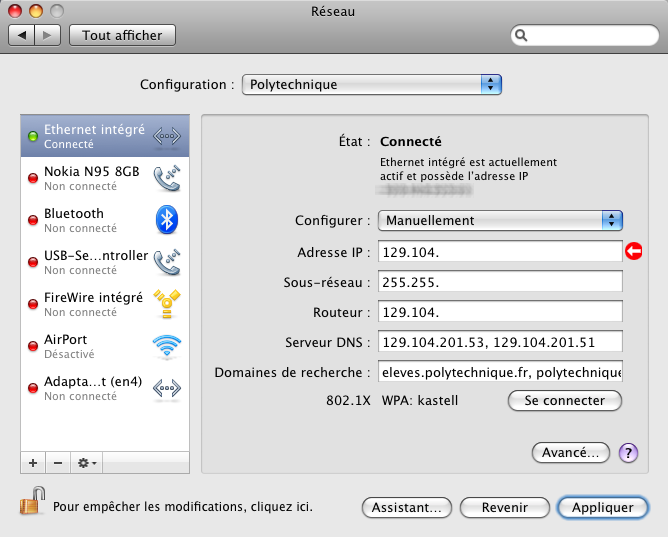
\includegraphics[width=0.96 \textwidth]{images/mac_config_ip_leopard}} \\
 		{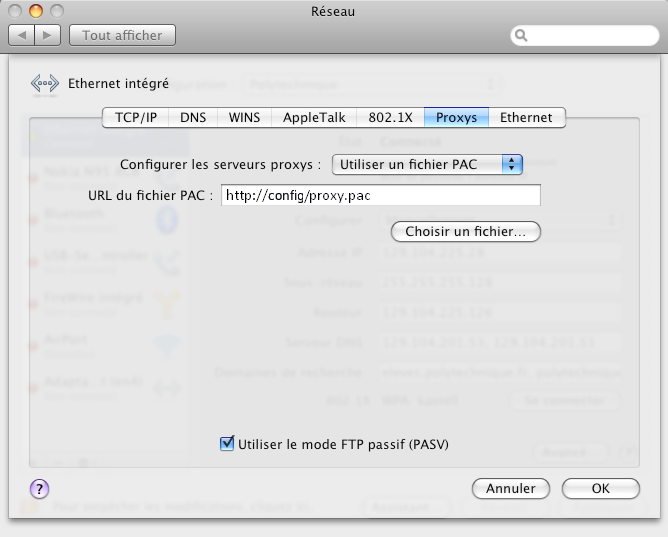
\includegraphics[width=0.96 \textwidth]{images/mac_config_proxy_leopard}}
\end{flushright}
 		\end{minipage}
 		 	\label{config:mac:ip:leopard}	}
     	 \caption{Cr\'eer une nouvelle configuration r\'eseau}

    \end{center}
  \end{figure*}

\pagebreak

La gestion des configurations r\'eseau de Mac OS X permet de cr\'eer plusieurs configurations et de passer en un clic de l'une  l'autre gr\^ace au sous-menu \menu{Configuration R\'eseau} du menu \menu{Pomme}. Cela est tr\`es pratique pour les machines vou\'ees \`a  \^etre connect\'ees \`a  plusieurs endroits successivement --- les portables par exemple (voir la page~\pageref{wifi} puis la section \emph{Wi-Fi} pour plus de pr\'ecisions sur le \emph{Wi-Fi}). Commence donc par cr\'eer une nouvelle configuration r\'eseau dans le menu d\'eroulant \menu{Configuration}.



Une fois la nouvelle configuration cr\'e\'ee, il faut configurer l'interface r\'eseau \emph{Ethernet}.



\app{Leopard} : Dans la colonne de gauche, s\'electionne \menu{Ethernet int\'egr\'e}.

Choisis alors \menu{Configurer IPv4} :% \menu{Manuellement} (\app{Tiger}) ou 
\menu{Configurer} : \menu{Manuellement} (\app{Leopard}). Tu trouveras toutes les valeurs d'adresses IP n\'ecessaires pour la configuration en page \pageref{calcul_ip} ou en te reportant aux captures d'\'ecran~\ref{config:mac:ip:leopard}. Si une partie d'adresse IP est blanche sur ces captures, c'est qu'elle t'est personnelle et que tu dois la calculer !


  
  

%\imageref{images/mac_config_ip_leopard}{0.4}{Configuration IP (Leopard)}{!ht}{config:mac:ip:leopard}}


Pour avoir acc\`es \`a  Internet, il faut aussi configurer le \emph{proxy}.

\app{Leopard} : Clique sur le bouton \menu{Avanc\'e...} puis sur l'onglet \menu{Proxys}.


\app{Mac OS X 10.3.3 et sup\'erieur} :  choisis l'option \menu{Configuration automatique de proxy} et indique \urllink{http://config/proxy.pac} comme URL de fichier PAC. Pour Mac OS X 10.3 \`a  10.3.2, n'oublie pas une fois que tu as le r\'eseau de faire la mise \`a  jour de ton syst\`eme, pour pouvoir configurer de fa\c con automatique le \emph{proxy}.

\app{Mac OS X 10.3.2 et inf\'erieur} : il te faut sp\'ecifier tous les
\emph{proxies} manuellement, et mettre \server{kuzh.polytechnique.fr}, port \server{8080}. Malheureusement, cele te permettra uniquement d'acc\'eder aux sites h\'eb\'erg\'es hors du pl\^atal : les sites \'el\`eves ne fonctionneront pas.


N'oublie pas d'activer le mode passif pour les transferts en FTP, en cochant la case comme dans la capture.

\subsubsection{Configuration antivirus}

Bien qu'il soit important de maintenir ton syst\`eme \`a  jour, un antivirus est pour l'instant tout \`a  fait superflu sur Mac, puisqu'aucun virus fonctionnel n'a encore vu le jour. Attention cependant, n'ouvre pas des fichiers dont tu ne te sois pas assur\'e de la provenance, et essaie de te tenir au courant des actualit\'es concernant les failles des applications que tu utilises.

\subsubsection{Configuration web}
\flimage{images/nux_firefox_icon}{0.07}{l}
Un point particulier pour la configuration du \emph{proxy} de \app{Firefox} : dans \menu{Pr\'ef\'erences}, \menu{Avanc\'e}, \menu{R\'eseau}, clique sur \menu{Param\`etres} et, dans le champ \menu{Adresse de configuration automatique du proxy}, inscris : \urllink{http://config/proxy.pac}. 
\\
\\

\flimage{images/mac_safari_icone}{0.07}{l}
\app{Safari}, le navigateur web d'Apple, est maintenant compatible avec la majorit\'e des sites \emph{web}. Tu peux donc t'en servir au quotidien, en faisant appel \`a  \app{Firefox} pour les sites r\'ecalcitrants. Un conseil : pense \`a  activer le blocage des fen\^etres \emph{pop-up} (dans le menu \menu{Safari}). \\
\\

\app{Google Chrome} se règle quant à lui automatiquement sur la configuration du système. 
\\

\subsubsection{Configuration \emph{mail}}
\flimage{images/mac_mail_icone}{0.07}{l} \app{Mail} : un client \emph{mail} offrant les fonctionnalit\'es classiques d'un bon client : recherche instantan\'ee, filtre antispam, r\`egles de tri automatique des \emph{mails}, regroupement des \emph{mails} correspondant \`a  une m\^eme discussion.

Au premier lancement, \app{Mail} te demandera de remplir les informations concernant ton compte \emph{mail} sur \server{poly}, il suffit de le remplir avec les donn\'ees suivantes :
\begin{description}
  \item[Nom complet] ton nom !
  \item[Adresse \'electronique] de la forme \mail{prenom.nom@polytechnique.edu}
  \item[Serveur de r\'eception] \server{poly.polytechnique.fr}
  \item[Type de compte] \menu{POP}
  \item[Nom d'utilisateur] ton \emph{login} \server{poly} (les huit premi\`eres lettres de ton nom en g\'en\'eral)
  \item[Mot de passe] ton mot de passe \server{poly}
  \item[Serveur d'envoi (SMTP)] \server{poly.polytechnique.fr} ou \server{ssl.polytechnique.org}
\end{description}

Si tu as d\'ej\`a  cr\'e\'e un compte pr\'ec\'edemment, il faut aller dans les \menu{Pr\'ef\'erences} (accessibles depuis le menu \menu{Mail}), onglet \menu{Comptes}, pour cr\'eer un autre compte en cliquant sur la case \menu{+}.

N'oublie pas de cocher \menu{Activer le cryptage SSL} dans l'onglet \menu{Avanc\'e}, port 995. Tu souhaiteras alors certainement installer le certificat de s\'ecurit\'e de \server{poly} (tu le trouveras sur \urllink{http://poly/}). Une fois que tu as t\'el\'echarg\'e le certificat, ouvre le fichier \menu{.CRT} obtenu, et dans \app{Trousseau d'acc\`es}, installe-le dans %\menu{X509Anchors} (Tiger) ou 
\menu{session} (Leopard).

Cette configuration marche pour acc\'eder \`a  ses mails depuis l'int\'erieur de l'X mais aussi de l'ext\'erieur, sans rien changer. En revanche tu ne peux pas envoyer de \emph{mails} depuis l'ext\'erieur , car le serveur \server{poly} ne le permet pas. Nous te conseillons vivement d'utiliser le serveur SMTP \server{polytechnique.org} et de regarder la configuration propos\'ee par \urllink{Polytechnique.org}. Celle-ci permet d'envoyer des \emph{mails} s\^urs \`a  l'ext\'erieur de l'\'Ecole sans modifier ta configuration par la suite. Tu peux ajouter ce SMTP dans l'onglet \menu{Comptes} des \menu{Pr\'ef\'erences} de \emph{mail} et r\'egler dans l'onglet \menu{Avanc\'es} comme dans la capture.

\begin{figure*}[!hl]
    \begin{center}
	      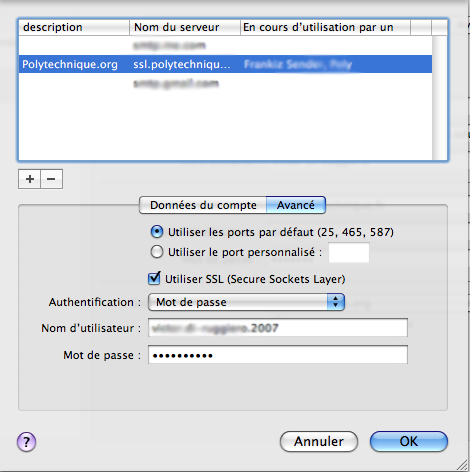
\includegraphics[width=0.4\textwidth]{images/mac_config_smtp_poltechnique.png} 
      \caption{Configurer le serveur SMTP \server{Polytechnique.org}}
    \end{center}
  \end{figure*}

%Le LDAP ne fonctionne pas \`a  l'heure actuelle avec \app{Mail} (mars 2009) sous \app{Leopard}, contrairement aux  autres syst\`emes d'exploitation (fonctionne cependant avec \app{Thunderbird}).
%\subsuEnfin, tu peux disposer dans \app{Mail} de l'annuaire de l'\`acole, mis \`a  disposition par la DSI. Pour cela, va dans les \menu{Pr\'ef\'erences} de Mail,
%puis dans la rubrique \menu{R\'edaction} et clique sur \menu{Configurer LDAP\ldots}. Tu peux ensuite utiliser le bouton \menu{+} pour ajouter un
%serveur, et remplir la fen\^etre comme sur la capture.

%\imagepos{images/mac_config_ldap}{0.6}{Configurer l'annuaire}{!ht}
%bsection{Logiciels additionnels}

%Les logiciels suivants sont utiles pour utiliser avec Mac OS X les services propos\'es sur le r\'eseau ; ils sont t\'el\'echargeables sur \server{frankiz}, dans la rubrique \menu{T\'el\'echarger}, \menu{Mac}.

%\subsubsection{Configuration \emph{news}}
%
%\flimage{images/mac_thunderbird_icone}{0.07}{l} 
%\app{Thunderbird} : un client \emph{news} permettant d'acc\'eder aux forums de discussion des \'el\`eves (voir page~\pageref{newsgroups} pour les d\'etails sur \server{frankiz}), mais aussi \`a  ceux de \server{usenet} gr\^ace au serveur \server{polynews.polytechnique.fr}. Il est tr\`es proche d'\app{Outlook Express} dans son esprit. Dans la m\^eme cat\'egorie, il existe \app{MacSOUP}, \app{Unison} ou encore \app{MT-NewsWatcher}. La configuration se fait de la m\^eme mani\`ere.
%
%Au premier lancement, l'application te propose d'importer les param\`etres depuis une autre application. Clique sur \menu{Suivant}. Tu peux alors choisir quel type de compte tu veux configurer (tu remarqueras que tu peux aussi cr\'eer un compte courrier \'electronique, et un compte RSS). S\'electionne \menu{Compte forums de discussion} et clique sur \menu{Suivant}. Entre alors les informations suivantes :
%
%\begin{description}
%  \item[Votre nom] ton nom ou ton pseudo
%  \item[Adresse de courrier] \mail{prenom.nom@polytechnique.edu}
%  \item[Serveur de forums] \server{news}
%  \item[Nom du compte] News Frankiz
%  \item[Nom d'utilisateur] ton \emph{login }poly (les huit premi\`eres lettres de ton nom en g\'en\'eral)
%  \item[Serveur d'envoi (SMTP)] \server{poly.polytechnique.fr} ou \server{ssl.polytechnique.org}
%\end{description}
%
%
%Pour t'abonner \`a  des groupes de discussion, il te suffit de s\'electionner le compte \menu{News Frankiz} dans la fen\^etre \menu{Dossiers} de \app{Thunderbird}, puis de cliquer sur \menu{G\'erer les abonnements aux groupes de discussion}. Tu pourras ensuite s\'electionner les forums qui t'int\'eressent parmi la liste propos\'ee. Reporte-toi \`a  la page \pageref{newsgroups} pour plus d'infos sur les \emph{newsgroups} auxquels t'abonner !
%

\subsubsection{Autres logiciels utiles}

%\flimage{images/mac_qrezix_icone}{0.07}{l} \app{qRezix} : en deux mots, c'est un programme d\'evelopp\'e par le BR pour faciliter la vie sur le r\'eseau. Tu peux le r\'ecup\'erer via le lien qRezix sur \server{Frankiz} ou sur \urllink{http://br.frankiz.net/qrezix/mac/}. Pour plus de d\'etails, voir le paragraphe consacr\'e \`a  qRezix \`a  la page \pageref{qrezix}. \\

%\app{Leopard} : le pare-feu se r\`egle pour chaque application; tu n'auras qu'\`a  r\'epondre \menu{Autoriser} lorsqu'il te demandera si tu veux \menu{Autoriser les connexions entrantes}.

%\noindent  \app{Tiger} : Attention, si ton \emph{firewall} est activ\'e, tu dois ouvrir les ports 5050, 5053 et 5055 en TCP. Pour cela va dans \app{Pr\'ef\'erences Syst\`eme}, dans le module \menu{S\'ecurit\'e}, onglet \menu{Coupe-feu}. S'il est \'ecrit \menu{Coupe-feu activ\'e}, clique le bouton \menu{Nouveau} et remplis la bo\^ite de dialogue comme sur la capture d'\'ecran ci-dessous pour ouvrir les ports.

%\imagepos{images/mac_firewall}{0.5}{Ouvrir les ports pour \app{qRezix} (Tiger)}{!ht}

%\flimage{images/mac_conversation_icone}{0.1}{l}
%\noindent\app{Colloquy}, un client IRC dans le m\^eme esprit qu'\app{iChat}. Il dispose d'une interface tr\`es simple ne n\'ecessitant pas de conna\^itre les commandes IRC. Tu peux te reporter \`a  la page \pageref{irc} pour plus d'infos sur l'IRC. \app{X-Chat Aqua} est un autre client IRC, plus riche en fonctionnalit\'es, mais moins agr\'eable \`a  utiliser. \\

%\flimage{images/mac_netnewswire_icone}{0.1}{l}
%\noindent\app{NetNewsWire} est la r\'ef\'erence des clients RSS sur Mac, et est maintenant gratuit. Dans le m\^eme genre, on peut citer \app{Vienna}, un client RSS open source, dont le d\'eveloppement actif est prometteur. Les flux RSS permettent d'agr\'eger dans un seul logiciel des informations en provenance de nombreux sites web, qui peuvent provenir de forums de discussions, de mises \`a  jour de logiciels, d'informations internationales\dots \\ \\

%\flimage{images/mac_fink_icone}{0.07}{l} \app{Fink} est la mani\`ere la plus simple d'installer sur Mac OS X nombre de logiciels issus du monde Unix (Linux par exemple). Gr\^ace \`a  lui, tu pourras installer les m\^emes logiciels que dans les salles informatiques. Par exemple, tu pourras installer Scilab sans trop de peine\dots La configuration n\'ecessaire se trouve sur la page \urllink{http://frankiz/binets/reseau/Miroir\_Fink}.\\ 

\flimage{images/logo_Windows}{0.1}{l}
 \app{Windows et les Mac Intel} : Maintenant il est possible d'installer Windows gr\^ace \`a  \app{Boot Camp}, livr\'e avec \app{Leopard}. Cela te permettra de profiter des quelques applications du monde PC qui valent le coup tout en gardant ton Mac. Tu peux \'egalement virtualiser Windows (utiliser Windows en utilisant en m\^eme temps Mac OS) gr\^ace \`a  \app{VMware Fusion}, \app{VirtualBox} ou \app{Parallels Desktop}. Le  d\'efaut de cette solution est que tu n'as pas d'acc\'el\'eration 3D, donc pour les jeux il te faudra red\'emarrer. Ces trois logiciels sont disponibles sur leurs sites \emph{web} respectifs. \`A toi de choisir !
Mais v\'erifie tout de m\^eme que tu as bien un processeur Intel (\menu{Pomme} puis s\'electionne \menu{\`A propos de ce Mac}).

\clearpage
